
The re-analysis above is observational: it characterizes one existing lineage and cannot,
on its own, establish that the \emph{amount} and \emph{composition} of biological data are what
drive the capability shift, rather than some idiosyncrasy of that particular CPT run. We
therefore ran a controlled experiment. Starting from the same vocabulary-expanded base (it-bio),
we trained seven fresh CPT models under a single fixed recipe, varying only the training-data
mixture, and evaluated all seven on the same axes. This turns the observational claim of
\S\ref{sec:results} into a causal one: mixture ratio is a controllable lever that shapes the
capability profile.

\paragraph{Controlled CPT protocol.} Each of the seven models continues pretraining from it-bio
for exactly $100$M tokens (QLoRA, $r{=}64$ over attention, MLP, and the MoE router, with
embeddings unfrozen --- identical to the BioCPT recipe of \S\ref{sec:setup}), on a single
96\,GB GPU. The \emph{only} independent variable is the data mixture. All sources are tokenized
once into per-source pools and sampled to the target ratio, so the token budget is held at
$100$M ($\pm0.003\%$) across every run. Two groups vary orthogonally:
\emph{(i)~Mixture ratio} --- the biological share of the corpus is set to $0/5/20/50\%$ (the
remainder English web text), with the biological portion held at a fixed internal composition
($70\%$ protein, $20\%$ DNA, $10\%$ biomedical literature); \emph{(ii)~Composition} --- the
biological share is fixed at $20\%$ and its \emph{content} is varied (protein-only, DNA-only,
protein+DNA), isolating which type of scientific data drives which capability. The 20\%-mixed
model (\texttt{M2-bio20}) serves as the shared protein+DNA+literature reference point for both
groups. Evaluation reuses the general axis (MMLU 5-shot, GSM8K 5-shot) and the biology axis
(protein homology, standard and remote; BixBench), scored by loglikelihood exactly as before.

\paragraph{Result 1: general capability is preserved across the whole mixture range.}
Table~\ref{tab:p2mix} and Figure~\ref{fig:p2mix} show that raising the biological share from
$0$ to $50\%$ costs essentially nothing on the general axis: MMLU moves $0.802\!\to\!0.796$
($-0.6$ pt) and GSM8K $0.873\!\to\!0.861$ ($-1.2$ pt) --- both within run-to-run noise. There is
no mixture threshold at which the general axis collapses; even a corpus that is half
out-of-distribution biological sequence leaves general knowledge and mathematical reasoning
intact. This is the causal counterpart of the ``no catastrophic forgetting'' observation of
\S\ref{sec:results}.

\paragraph{Result 2: biological capability rises monotonically with biological share.}
Over the same sweep the biology axis climbs steadily: protein-homology discrimination (standard)
rises from MCC $0.228$ to $0.375$ ($+65\%$), remote homology --- the harder, low-identity
regime --- flips from below chance to positive ($-0.023\!\to\!+0.088$), and BixBench saturates
($0.850\!\to\!1.000$). The general axis is flat and the biology axis is monotone increasing over
the same models: the two do not trade off. Figure~\ref{fig:p2traj} plots the joint trajectory,
the two-dimensional form of the capability-shaping curve.

\begin{table*}[t]\centering\small
\caption{Controlled mixture sweep from it-bio ($100$M tokens each, single fixed recipe).
Raising biological share preserves the general axis (MMLU, GSM8K) while monotonically lifting
the biology axis. All values loglikelihood-scored; homology/BixBench are MCC.}
\label{tab:p2mix}
\begin{tabular}{lccccccc}
\toprule
Model & Bio\% & MMLU & GSM8K & TruthQA & Homology-std & Homology-rem & BixBench \\
\midrule
\texttt{M0-base}  & 0  & \textbf{0.802} & \textbf{0.873} & 0.545 & 0.228 & $-0.023$ & 0.850 \\
\texttt{M1-bio5}  & 5  & 0.801 & 0.867 & 0.524 & 0.270 & $-0.055$ & 0.882 \\
\texttt{M2-bio20} & 20 & 0.800 & 0.867 & 0.521 & 0.217 & $-0.074$ & \textbf{1.000} \\
\texttt{M3-bio50} & 50 & 0.796 & 0.861 & 0.519 & \textbf{0.375} & \textbf{0.088} & \textbf{1.000} \\
\bottomrule
\end{tabular}
\end{table*}

\begin{figure}[h]\centering
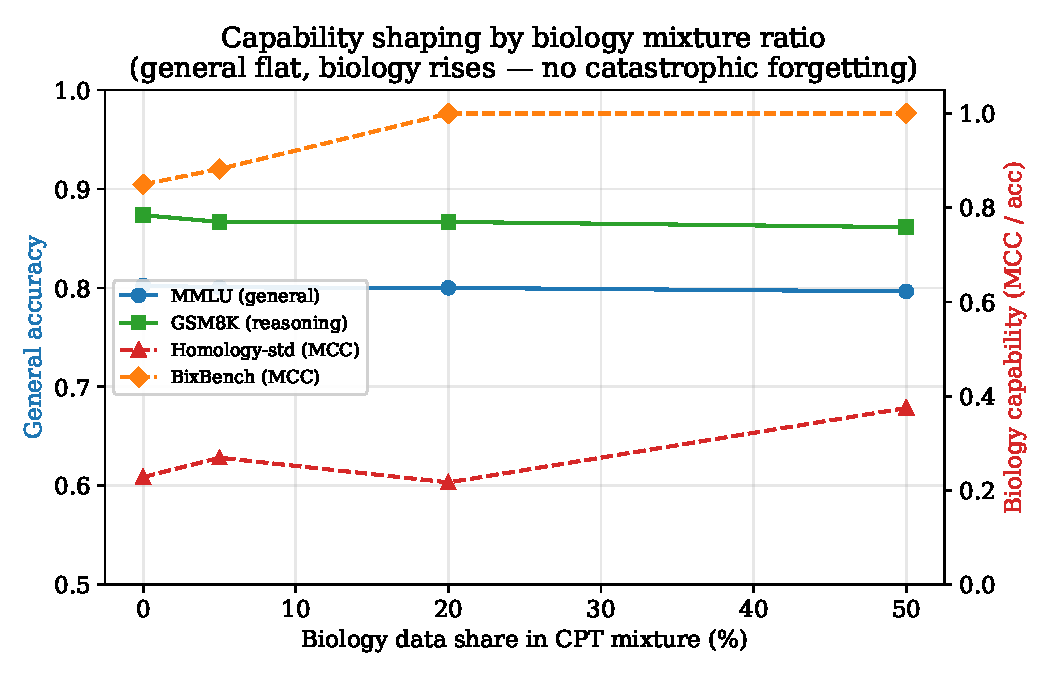
\includegraphics[width=0.78\linewidth]{figs/p2_fig1_mixture.pdf}
\caption{Capability shaping by biological mixture ratio. As the biological share of a fixed
$100$M-token CPT corpus rises from $0$ to $50\%$, the general axis (MMLU, GSM8K; left scale)
stays flat while the biology axis (homology MCC, BixBench MCC; right scale) rises --- controlled
evidence that mixture ratio shapes the capability profile without a forgetting penalty.}
\label{fig:p2mix}
\end{figure}

\paragraph{Result 3: different scientific data shape different capabilities.}
Holding the biological share at $20\%$ and varying its content (Table~\ref{tab:p2comp},
Figure~\ref{fig:p2comp}) reveals that the \emph{type} of scientific data matters and is not
interchangeable. DNA is most effective for \emph{remote} homology (MCC $+0.043$, versus
$-0.004$ for protein-only), whereas protein sequence is strongest on BixBench ($0.966$) and
standard homology; the protein+DNA mix is intermediate. The composition of a scientific-data
corpus is thus a second, finer lever: not only \emph{how much} scientific data, but \emph{which}
kind, selects which downstream capability is amplified.

\begin{table}[h]\centering\small
\caption{Composition ablation at fixed $20\%$ biological share. Different scientific-data types
amplify different biological capabilities. MCC; \texttt{M2-bio20} = protein+DNA+literature.}
\label{tab:p2comp}
\begin{tabular}{lccc}
\toprule
Model & Homology-std & Homology-rem & BixBench \\
\midrule
\texttt{C1-protein}  & 0.247 & $-0.004$ & \textbf{0.966} \\
\texttt{C2-dna}      & \textbf{0.312} & \textbf{0.043} & 0.850 \\
\texttt{C3-protdna}  & 0.237 & 0.025 & 0.914 \\
\texttt{M2-bio20}\,(+lit) & 0.217 & $-0.074$ & \textbf{1.000} \\
\bottomrule
\end{tabular}
\end{table}

\begin{figure}[h]\centering
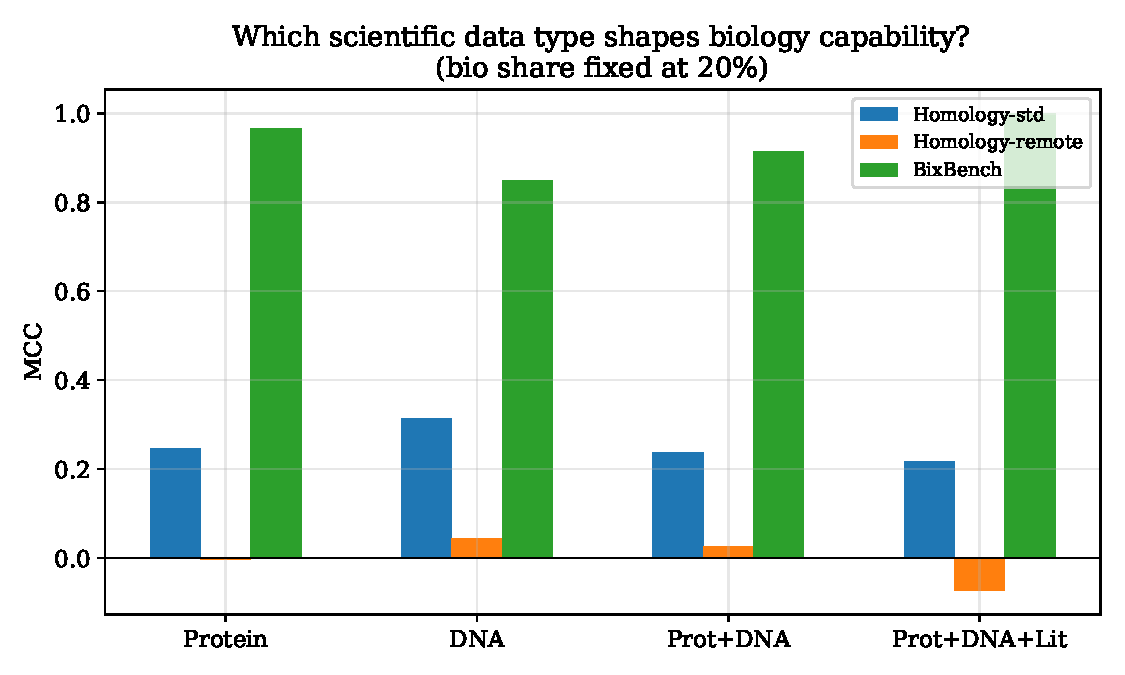
\includegraphics[width=0.72\linewidth]{figs/p2_fig2_composition.pdf}
\caption{Composition ablation (biological share fixed at $20\%$). DNA most improves remote
homology; protein most improves BixBench and standard homology --- the type of scientific data,
not just its quantity, selects which capability is shaped.}
\label{fig:p2comp}
\end{figure}

\begin{figure}[h]\centering
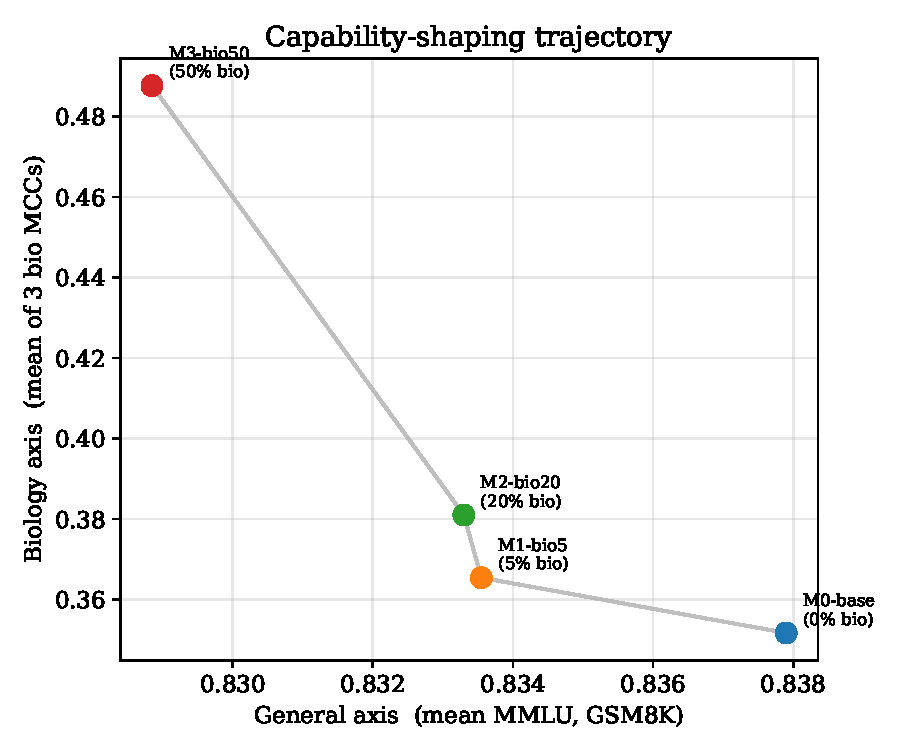
\includegraphics[width=0.56\linewidth]{figs/p2_fig3_shaping2d.pdf}
\caption{Two-dimensional capability-shaping trajectory of the mixture sweep. Each point is one
CPT model; increasing biological share moves the model up the biology axis with negligible
displacement along the general axis.}
\label{fig:p2traj}
\end{figure}
